\PassOptionsToPackage{unicode}{hyperref}
\PassOptionsToPackage{hyphens}{url}
%
\documentclass[
  11pt,
  answers  
]{exam}
\usepackage[fleqn]{amsmath}
\usepackage[]{plex-otf}
\usepackage{iftex}
\usepackage[a4paper, margin=2.5cm]{geometry}
\usepackage{graphicx}
% \ifPDFTeX
%   \usepackage[T1]{fontenc}
%   \usepackage[utf8]{inputenc}
%   \usepackage{textcomp} % provide euro and other symbols
% \else % if luatex or xetex
%   \usepackage{unicode-math}
%   \defaultfontfeatures{Scale=MatchLowercase}
%   \defaultfontfeatures[\rmfamily]{Ligatures=TeX,Scale=1}
% \fi
% Use upquote if available, for straight quotes in verbatim environments
\IfFileExists{upquote.sty}{\usepackage{upquote}}{}
\IfFileExists{microtype.sty}{% use microtype if available
  \usepackage[]{microtype}
  \UseMicrotypeSet[protrusion]{basicmath} % disable protrusion for tt fonts
}{}
\makeatletter
\makeatother
\usepackage{xcolor}
\IfFileExists{xurl.sty}{\usepackage{xurl}}{} % add URL line breaks if available
\IfFileExists{bookmark.sty}{\usepackage{bookmark}}{\usepackage{hyperref}}
\urlstyle{same} % disable monospaced font for URLs
\setlength{\emergencystretch}{3em} % prevent overfull lines
\providecommand{\tightlist}{%
  \setlength{\itemsep}{0pt}\setlength{\parskip}{0pt}}
\setcounter{secnumdepth}{-\maxdimen} % remove section numbering
\newlength{\cslhangindent}
\setlength{\cslhangindent}{1.5em}
\newlength{\csllabelwidth}
\setlength{\csllabelwidth}{3em}
\newlength{\cslentryspacingunit} % times entry-spacing
\setlength{\cslentryspacingunit}{\parskip}
\newenvironment{CSLReferences}[2] % #1 hanging-ident, #2 entry spacing
 {% don't indent paragraphs
  \setlength{\parindent}{0pt}
  % turn on hanging indent if param 1 is 1
  \ifodd #1
  \let\oldpar\par
  \def\par{\hangindent=\cslhangindent\oldpar}
  \fi
  % set entry spacing
  \setlength{\parskip}{#2\cslentryspacingunit}
 }%
 {}
\usepackage{calc}
\newcommand{\CSLBlock}[1]{#1\hfill\break}
\newcommand{\CSLLeftMargin}[1]{\parbox[t]{\csllabelwidth}{#1}}
\newcommand{\CSLRightInline}[1]{\parbox[t]{\linewidth - \csllabelwidth}{#1}\break}
\newcommand{\CSLIndent}[1]{\hspace{\cslhangindent}#1}
\ifLuaTeX
  \usepackage{selnolig}  % disable illegal ligatures
\fi
\renewcommand{\solutiontitle}{\noindent\textbf{Jawab:}\par\noindent}
\newcommand{\mytitle}{Programming Fundamentals (IF 130)}
\newcommand{\theauthor}{Rivo Juicer Wowor}
\newcommand{\affiliation}{00000059635}

% \title{\textbf{\mytitle}}
% \author{\theauthor \
		% \small{\affiliation}}
% \date{}

% \usepackage{fancyhdr}
\lhead{\footnotesize{\textbf{\mytitle}}}%
\rfoot{\thepage}%
\cfoot{}
\lfoot{\footnotesize{\theauthor \hspace{1pt} (\affiliation)}}
\pagestyle{headandfoot}

% \pagestyle{plain}
\setlength{\parindent}{2em}
\renewcommand{\baselinestretch}{1.5}
\hbadness=99999
\usepackage{enumitem}
\unframedsolutions

\usepackage{graphicx}
\usepackage{listings}
\lstdefinestyle{mystyle}{
	showtabs=false,                  
  tabsize=3,
	basicstyle=\linespread{0.6},
  breaklines=true,
  postbreak=\mbox{\textcolor{red}{$\hookrightarrow$}\space},
  keywordstyle=\color{black}\bfseries,
  keywords={ ,BEGIN, START, END, DECLARE, SET, PROMPT, GET, PRINT, IF, ENDIF, ELSE, BREAK, RETURN, WHILE, ENDWHILE, DO, UNTIL, FOR, CASE, ENDCASE, ENDFOR, Display, NOT, &&, ||, },
}
\lstset{style=mystyle}

\begin{document}
	% \begin{titlepage}
	% 	\centering
	% 	\vspace{2cm}
	% 	
\includegraphics[width=0.5\textwidth]{../../ref/logoUMN.png}\par\vspace{1cm}
	% 	\vspace{1.5cm}
	% 	\Large{Midterm Assignment} \par
	% 	\vspace{1cm}
	% 	\huge{\textbf{\mytitle}} \par
	% 	\vspace{1.5cm}
	% 	\Large{\theauthor} \par
	% 	\emph{\affiliation} \par
	% 	\vfill
	% 	\today
	% \end{titlepage}	

  \begin{questions}
    \question
    \begin{solution}
      \begin{lstlisting}
bayarParkir
START
	DECLARE platNomor, durasiParkir, tanggalParkir, platGanjilOrGenap
1	PROMPT "Plat nomor (Isi angka saja): "
	GET platNomor
2	PROMPT "Lamanya Parkir (dalam jam): "
	GET durasiParkir
3	PROMPT "Tanggal Hari ini: "
	GET tanggalParkir

4	platGanjilOrGenap = platNomor % 2
5	tanggalGanjilOrGenap = tanggalParkir % 2

6	total = penentuanBiaya(platGanjilOrGenap, durasiParkir, tanggalGanjilOrGenap)
7	PRINT "Total biaya: " + total
END

penentuanBiaya(plat, durasi, tanggal)
START
	DECLARE totalTarif
1	CASE of durasi:
		1: IF (plat == 0 AND tanggal == 0)
			totalTarif = 5000
		   ELSE IF (plat != 0 AND tanggal != 0)
			totalTarif = 6000
		   ELSE
			totalTarif = 5000	
		   ENDIF
		   BREAK
		>1: IF (plat == 0 AND tanggal == 0)
			totalTarif = 5000 + (3000 * durasi)
		    ELSE IF (plat != 0 AND tanggal != 0)
		        totalTarif = 6000 + (2000 * durasi)
		    ELSE
			totalTarif = 5000 + (4000 * durasi)
		    ENDIF
		    BREAK
	ENDCASE	
	
2	IF (totalTarif > 40000 AND ((plat == 0 AND tanggal == 0) OR (plat != 0 AND tanggal != 0)))
		totalTarif = 40000
	ELSE IF (totalTarif > 50000)
		totalTarif = 50000
	ENDIF
	RETURN totalTarif
END
      \end{lstlisting}
      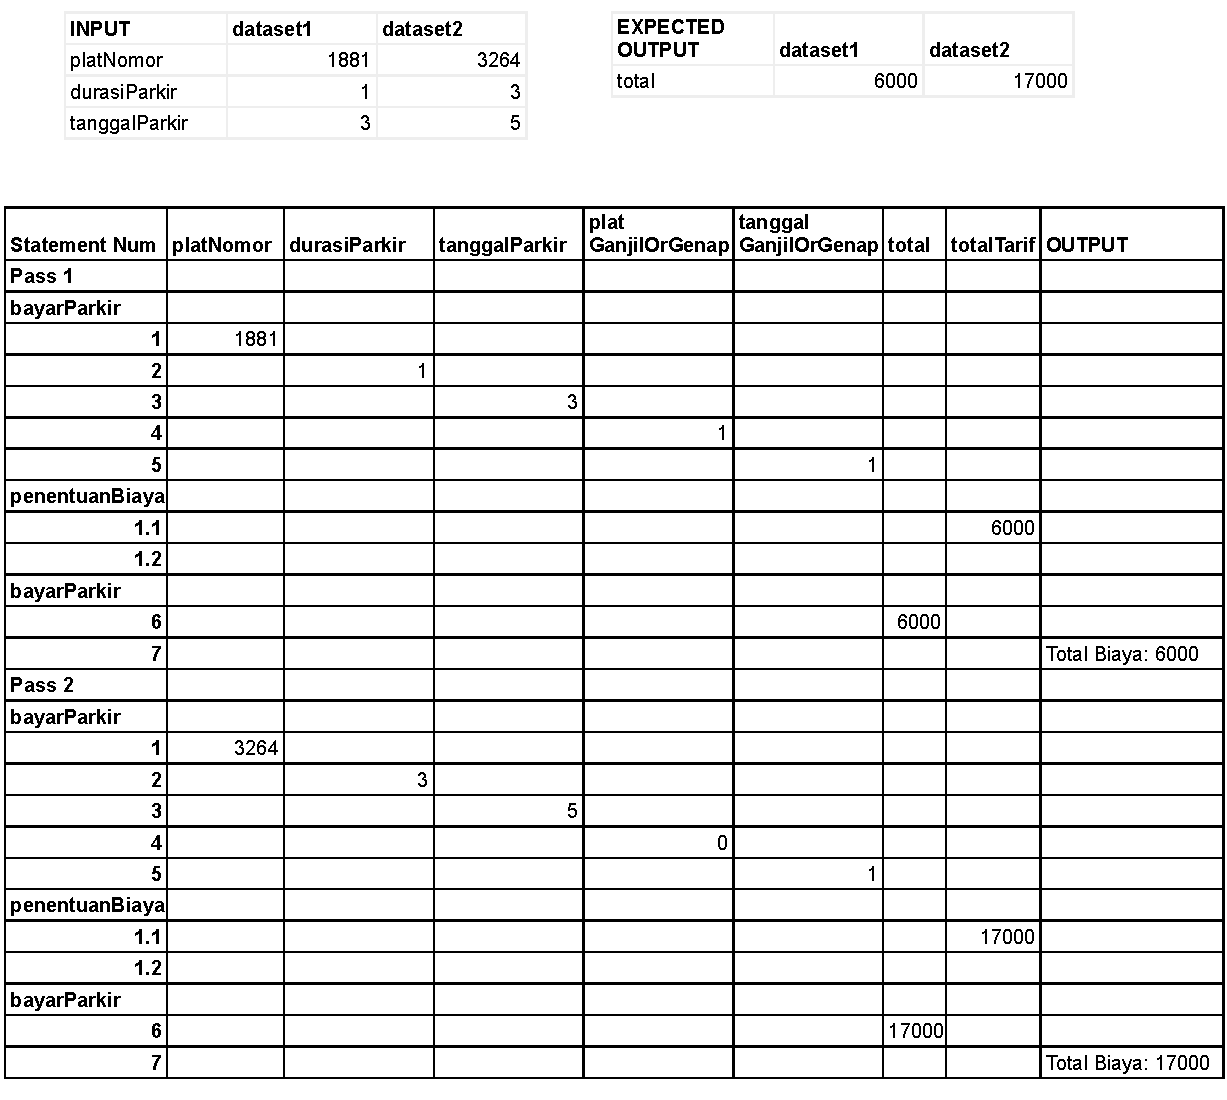
\includegraphics[clip,scale=0.8]{pdf/nomor1.pdf}
    \end{solution}
    \pagebreak
    \question
    \begin{solution}
      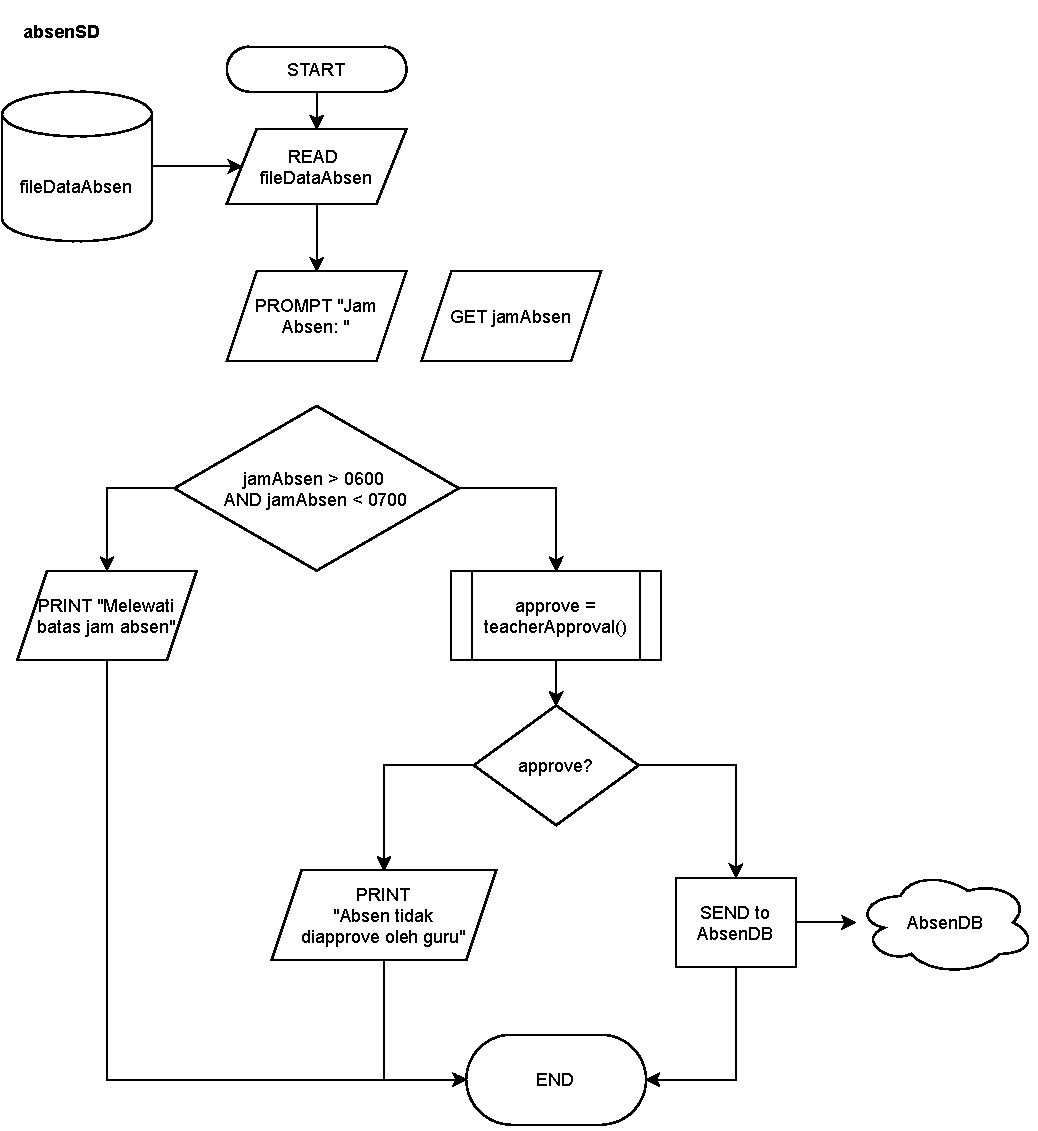
\includegraphics[clip,scale=0.8]{pdf/nomor2.pdf}
    \end{solution}
    \pagebreak
    \question
    \begin{solution}
      \begin{lstlisting}
simpanDataSiswa
START
	DECLARE INT jumlah
	DECLARE STRING keepGoing
	DECLARE ARRAY dataSiswa
	DO
		dataSiswa[jumlah] = inputData()
		jumlah++
		PROMPT "Isi lagi? (Y/n): "
		GET keepGoing
		IF (keepGoing == y)
			keepGoing == TRUE
		ELSE IF (keepGoing == n) 
			keepGoing == FALSE
		ENDIF
	WHILE (keepGoing != FALSE)
	FOR (int i = 0; i < jumlah; i++)
		FOR (int j = 0; j < jumlah; j++)
			IF (dataSiswa[i][0] == dataSiswa[j][0])
				PRINT "Terdapat duplikat data"
			ENDIF
		ENDFOR
	ENDFOR
	PRINT "Pengisian data selesai"
	PRINT "Jumlah siswa pada data: ", jumlah
END

inputData
START
	DECLARE ARRAY siswa
	PROMPT "Nama: "
	GET siswa[0]
	PROMPT "Kelas (A/B/C): "
	GET siswa[1]
	RETURN siswa 
END
      \end{lstlisting}
    \end{solution}
  \end{questions}
\end{document}
